\section{Datenverarbeitung}\label{sec:Datenverarbeitung}
Die Bewertung des Systemzustands erfolgt über die ermittelung von drei zentralen Kennwerten. Zum muss der Aktuelle Systemzustand ermittelt weerden. Dieser ist eine Momentaufnahme, die innerhalb der Letzen Minute erfasst wird. Dieser bildet das Kernelement der bewertung. Alle weiteren Kennwerte bauen auf dem Aktuellen Systemzustand auf. Im weiteren verlauf wird dieser als \textit{SytemStatus} betietelt. Desweiteren wird aus den aufzeichnungen des \textit{SystesmStatus} der sogenante \textit{HistorySystemStatus} ermittelt. Dieser Liefert eine historische Einsicht in das Nutzungsverhalten des Systems über eine gewisse Zeit. Zuletzt kann über den \textit{HistorySystemStatus} die, in Abschnitt \ref{sec:MTBF} behandelten, Systemzuverlässigkeit errechnet werden.

\newpage
\subsection{Health Status Definition}
\begin{wrapfigure}{r}{0.2\textwidth}
    \vspace{-1.2cm}
    \begin{center}
      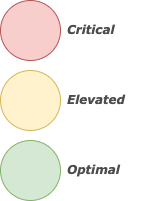
\includegraphics[width=0.2\textwidth]{HealthStatus.png}
    \end{center}
    \vspace{-0.5cm}
    \caption{}
    \label{fig:Systemstatus}
    \vspace{-0.5cm}
\end{wrapfigure}
Der Betrieb der Zielplatform wird zunächst in drei Zustände unterteilt. Sind alle Temperatur und die CPU Auslastung in der Norm, so läuft die Platform im \textit{Optimal} bereich. Steigen Temperaturen oder CPU Auslastung, so steigt der Status auf \textit{Elevated}. Erreicht die Temperatur nun grenzwerte die nich überschritten werden dürfen, begibt sich der SystemStatus in den \textit{Critical} Bereich.\\
Der \textit{Systemstatus} wird daher in die drei Zustände \textit{Optimal}, \textit{Elevated} und \textit{Critical} unterteilt. Der SystemStatus kann, wie in  Abbildung \ref{fig:Systemstatus}, nach dem Ampel Prinzip visualisiert.\\
Die Algorithmen zur ermitteung dieser Werte sind unabhängig von der Hardwarekonfiguration der verschiedenen Zielplatformen. Lediglich die verwendeten Daten die den Algorithmen zur verfügung gestellt werden unterscheiden sich für jede Platform. In den folgenden Abschnitten werden die Algorithmen auf die VisuNet FLX Platform ausgelegt. Dabei wird die Architektur so ausgelegt, das sie für alle anderen Platformen verwendbar ist.
  
\subsubsection*{Hardwarekonfiguration der VisuNet FLX Platform}
Damit die Ergebnisse der Bewertungsalgorithmen möglichst genau sind, ist es wichtig mit den Richigen Werten zu rechnen. Zum einen müssen die richigen Temperaturgrenzen für das System festgelegt werden. 
\begin{center}
    \begin{figure}[h!]
        \centering
        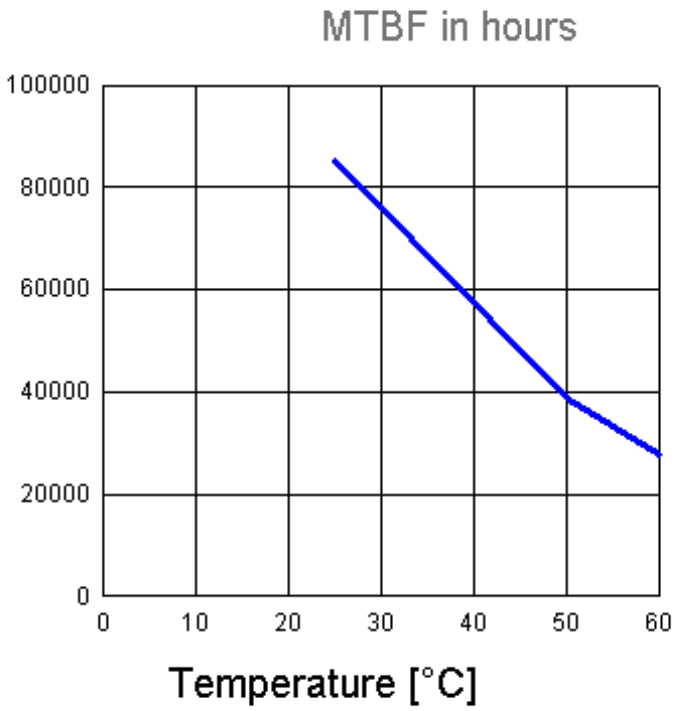
\includegraphics[width=0.3\textwidth]{FLXMTBFPrediction}
        \caption{\ac{mtbf} Voirhersage für die VisuNet FLX Platform}
        \label{fig:FLXMTBF}
    \end{figure}
\end{center}
\vspace{-1.8cm}
Die aus Anhang \ref{app:mtbfprediction} entnommene Abbildung \ref{fig:FLXMTBF} stellt den \ac{mtbf} ,der VisuNet FLX Platform, in Abhängigkeit zur Betriebstemperatur des Gerätes. Aus dieser werden drei Intervalle für den Betrieb des 
Gerätes festgelegt. Von 0°C bis 45°C läuft das Gerät im \textit{Optimal} Betrieb. Dabei wird für dieses Interval eine \ac{mtbf} von 60000h angenommen. Im zweiten Intervall von 45°C bis 63°C läuft das Geräte im \textit{Elevated} betrieb. Der angenommene \ac{mtbf} für dieses Intervall ist 40000h. Bei allem über 63°C läuft das Gerät im \textit{Critical} betrieb, mit einem \ac{mtbf} 30000h.\\
\\
Um die \ac{mtbf} Vorhersage aus Abbildung \ref{fig:FLXMTBF} mit den Temperaturen der Hardware verwenden zu können, müssen hierfür die richtigen Sensoren verwendet werden. Abbuldung \ref{fig:FLXSensoren} Zeigt die Sensorverteilung auf der VisuNet FLX Platform. Da CPU und Spannungsregulator (Siehe Abb. \ref{fig:FLXSensoren} \textit{VR VCC Temperature} und \textit{CPU Temperature}) zwei Signifikante Hitzequellen sind, wird der Sensor \textit{Temperatur 1} zur bestimmung der Betriebstemperatur gewählt. 
\begin{center}
    \begin{figure}[h!]
        \centering
        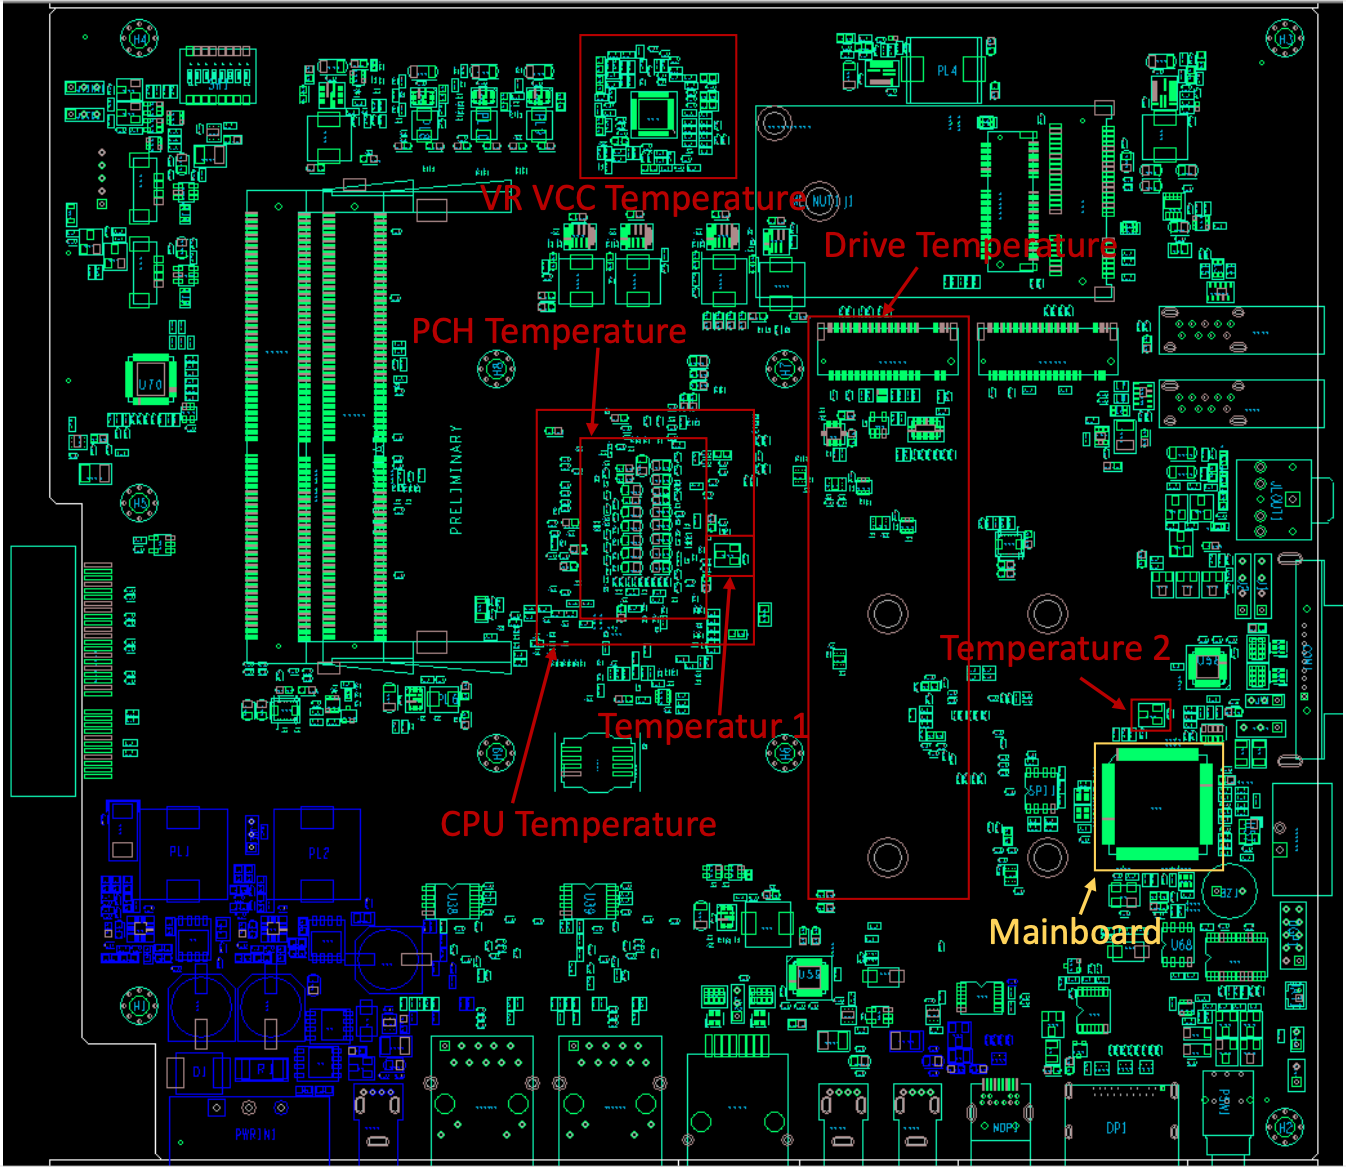
\includegraphics[width=0.7\textwidth]{FLXSensorPlatzierung}
        \caption{Sensorverteilung auf der Mainboard Platine der VisuNet FLX Platform}
        \label{fig:FLXSensoren}
    \end{figure}
\end{center}
\vspace{-1.8cm}  
\todo{Temperatur 1 typo korregieren}

\subsection{Ermittelung des SystemStatus}
Der \textit{SystemStatus} wird mithilfe des, in Abschnit \ref{sec:FuzzyLogic} beschriebenen, FuzzyLogic Verfahren ermittelt. Hierfür müssen zunächst die Linguistische Variablen festgelegt werden. Hierzu wird für jeden Eingang des Systems eine linguistische Variable und die dazugehörigen \textit{Membershipfunktion} festgelegt.  


\subsection{Ermittelung der Systemstatus Historie}
\subsection{Ermittelung der Systemzuverlässigkeit}